
% --- LaTeX Homework Template - S. Venkatraman ---

% --- Set document class and font size ---

\documentclass[letterpaper, 11pt]{article}

% --- Package imports ---

\usepackage{
  booktabs, amsmath, amsthm, amssymb, mathtools,	  % Math typesetting
  graphicx, wrapfig, subfig, float,                  % Figures and graphics formatting
  listings, color,  pythonhighlight,     % Code formatting
  fancyhdr, sectsty, hyperref, enumerate, enumitem } % Headers/footers, section fonts, links, lists

% --- Page layout settings ---

% Set page margins
\usepackage[left=1in, right=1in, bottom=1in, top=1.1in, headsep=0.2in]{geometry}

% Anchor footnotes to the bottom of the page
\usepackage[bottom]{footmisc}

% Set line spacing
\renewcommand{\baselinestretch}{1.2}

% Set spacing between paragraphs
\setlength{\parskip}{1.5mm}

% Allow multi-line equations to break onto the next page
\allowdisplaybreaks

% Enumerated lists: make numbers flush left, with parentheses around them
\setlist[enumerate]{wide=0pt, leftmargin=21pt, labelwidth=0pt, align=left}
\setenumerate[1]{label={(\arabic*)}}

% --- Page formatting settings ---

% Set link colors for labeled items (blue) and citations (red)
\hypersetup{colorlinks=true, linkcolor=blue, citecolor=red}

% Make reference section title font smaller
\renewcommand{\refname}{\large\bf{References}}

% --- Settings for printing computer code ---

% Define colors for green text (comments), grey text (line numbers),
% and green frame around code
\definecolor{greenText}{rgb}{0.5, 0.7, 0.5}
\definecolor{greyText}{rgb}{0.5, 0.5, 0.5}
\definecolor{codeFrame}{rgb}{0.5, 0.7, 0.5}

% Define code settings
\lstdefinestyle{code} {
  frame=single, rulecolor=\color{codeFrame},            % Include a green frame around the code
  numbers=left,                                         % Include line numbers
  numbersep=8pt,                                        % Add space between line numbers and frame
  numberstyle=\tiny\color{greyText},                    % Line number font size (tiny) and color (grey)
  commentstyle=\color{greenText},                       % Put comments in green text
  basicstyle=\linespread{1.1}\ttfamily\footnotesize,    % Set code line spacing
  keywordstyle=\ttfamily\footnotesize,                  % No special formatting for keywords
  showstringspaces=false,                               % No marks for spaces
  xleftmargin=1.95em,                                   % Align code frame with main text
  framexleftmargin=1.6em,                               % Extend frame left margin to include line numbers
  breaklines=true,                                      % Wrap long lines of code
  postbreak=\mbox{\textcolor{greenText}{$\hookrightarrow$}\space} % Mark wrapped lines with an arrow
}

% Set all code listings to be styled with the above settings
\lstset{style=code}

% --- Math/Statistics commands ---

% Add a reference number to a single line of a multi-line equation
% Usage: "\numberthis\label{labelNameHere}" in an align or gather environment
\newcommand\numberthis{\addtocounter{equation}{1}\tag{\theequation}}

% Shortcut for bold text in math mode, e.g. $\b{X}$
\let\b\mathbf

% Shortcut for bold Greek letters, e.g. $\bg{\beta}$
\let\bg\boldsymbol

% Shortcut for calligraphic script, e.g. %\mc{M}$
\let\mc\mathcal

% \mathscr{(letter here)} is sometimes used to denote vector spaces
\usepackage[mathscr]{euscript}

% Convergence: right arrow with optional text on top
% E.g. $\converge[w]$ for weak convergence
\newcommand{\converge}[1][]{\xrightarrow{#1}}

% Normal distribution: arguments are the mean and variance
% E.g. $\normal{\mu}{\sigma}$
\newcommand{\normal}[2]{\mathcal{N}\left(#1,#2\right)}

% Uniform distribution: arguments are the left and right endpoints
% E.g. $\unif{0}{1}$
\newcommand{\unif}[2]{\text{Uniform}(#1,#2)}

% Independent and identically distributed random variables
% E.g. $ X_1,...,X_n \iid \normal{0}{1}$
\newcommand{\iid}{\stackrel{\smash{\text{iid}}}{\sim}}

% Equality: equals sign with optional text on top
% E.g. $X \equals[d] Y$ for equality in distribution
\newcommand{\equals}[1][]{\stackrel{\smash{#1}}{=}}

% Math mode symbols for common sets and spaces. Example usage: $\R$
\newcommand{\R}{\mathbb{R}}   % Real numbers
\newcommand{\C}{\mathbb{C}}   % Complex numbers
\newcommand{\Q}{\mathbb{Q}}   % Rational numbers
\newcommand{\Z}{\mathbb{Z}}   % Integers
\newcommand{\N}{\mathbb{N}}   % Natural numbers
\newcommand{\F}{\mathcal{F}}  % Calligraphic F for a sigma algebra
\newcommand{\El}{\mathcal{L}} % Calligraphic L, e.g. for L^p spaces

% Math mode symbols for probability
\newcommand{\pr}{\mathbb{P}}    % Probability measure
\newcommand{\E}{\mathbb{E}}     % Expectation, e.g. $\E(X)$
\newcommand{\var}{\text{Var}}   % Variance, e.g. $\var(X)$
\newcommand{\cov}{\text{Cov}}   % Covariance, e.g. $\cov(X,Y)$
\newcommand{\corr}{\text{Corr}} % Correlation, e.g. $\corr(X,Y)$
\newcommand{\B}{\mathcal{B}}    % Borel sigma-algebra

% Other miscellaneous symbols
\newcommand{\tth}{\text{th}}	% Non-italicized 'th', e.g. $n^\tth$
\newcommand{\Oh}{\mathcal{O}}	% Big-O notation, e.g. $\O(n)$
\newcommand{\1}{\mathds{1}}	% Indicator function, e.g. $\1_A$

% Additional commands for math mode
\DeclareMathOperator*{\argmax}{argmax}    % Argmax, e.g. $\argmax_{x\in[0,1]} f(x)$
\DeclareMathOperator*{\argmin}{argmin}    % Argmin, e.g. $\argmin_{x\in[0,1]} f(x)$
\DeclareMathOperator*{\spann}{Span}       % Span, e.g. $\spann\{X_1,...,X_n\}$
\DeclareMathOperator*{\bias}{Bias}        % Bias, e.g. $\bias(\hat\theta)$
\DeclareMathOperator*{\ran}{ran}          % Range of an operator, e.g. $\ran(T) 
\DeclareMathOperator*{\dv}{d\!}           % Non-italicized 'with respect to', e.g. $\int f(x) \dv x$
\DeclareMathOperator*{\diag}{diag}        % Diagonal of a matrix, e.g. $\diag(M)$
\DeclareMathOperator*{\trace}{trace}      % Trace of a matrix, e.g. $\trace(M)$

% Numbered theorem, lemma, etc. settings - e.g., a definition, lemma, and theorem appearing in that 
% order in Section 2 will be numbered Definition 2.1, Lemma 2.2, Theorem 2.3. 
% Example usage: \begin{theorem}[Name of theorem] Theorem statement \end{theorem}
\theoremstyle{definition}
\newtheorem{theorem}{Theorem}[section]
\newtheorem{proposition}[theorem]{Proposition}
\newtheorem{lemma}[theorem]{Lemma}
\newtheorem{corollary}[theorem]{Corollary}
\newtheorem{definition}[theorem]{Definition}
\newtheorem{example}[theorem]{Example}
\newtheorem{remark}[theorem]{Remark}
\usepackage{booktabs}
\usepackage{caption}
\usepackage{array}
% Un-numbered theorem, lemma, etc. settings
% Example usage: \begin{lemma*}[Name of lemma] Lemma statement \end{lemma*}
\newtheorem*{theorem*}{Theorem}
\newtheorem*{proposition*}{Proposition}
\newtheorem*{lemma*}{Lemma}
\newtheorem*{corollary*}{Corollary}
\newtheorem*{definition*}{Definition}
\newtheorem*{example*}{Example}
\newtheorem*{remark*}{Remark}
\newtheorem*{claim}{Claim}

% --- Left/right header text (to appear on every page) ---

% Include a line underneath the header, no footer line
\pagestyle{fancy}
\renewcommand{\footrulewidth}{0pt}
\renewcommand{\headrulewidth}{0.4pt}

% Left header text: course name/assignment number
\lhead{OMIS 338 (Principles of Operations Management) -- Write-Up 12}

% Right header text: your name
\rhead{Matt Warner}

% --- Document starts here ---

\begin{document}
\subsection*{Problem 16-57}
Given the following cost-of-quality data:
\begin{table}[H]
\centering
\begin{tabular}{@{}p{10cm}r@{}}
\toprule
\textbf{Quality Cost} & \textbf{Amount (\$)} \\ \midrule
\multicolumn{2}{l}{\textbf{Loan Processing}} \\ \midrule
Run credit checks & 2,409.32 \\
Review documents & 3,181.80 \\
Make document corrections; gather additional information & 1,333.50 \\
Prepare tickler file; review and follow up on titles, 
insurance, second meetings & 167.95 \\
Review all output & 2,676.44 \\
Correct rejects and incorrect output & 438.05 \\
Reconcile incomplete collateral report & 74.34 \\
Handle dealer problem calls; address associate problems; 
research and communicate information & 2,360.00 \\
Compensate for system downtime & 526.74 \\
Conduct training & 1,235.00 \\ \midrule
\multicolumn{2}{l}{\textbf{Loan Payment}} \\ \midrule
Receive, inspect, and process payments & 830.00 \\
Respond to inquiries when no coupon is presented with payments & 849.75 \\ \midrule
\multicolumn{2}{l}{\textbf{Loan Payoff}} \\ \midrule
Receive, inspect, and process payoff and release documents & 296.26 \\
Research payoff problems & 15.77 \\ \bottomrule
\end{tabular}
\end{table}
\noindent We can classify these into the appropriate cost-of-quality categories: appraisal, internal failure and external failure. Using the definitions for the four categories, we have:

\begin{table}[H]
\centering
\begin{tabular}{@{}p{10cm}r@{}}
\toprule
\textbf{Quality Cost} & \textbf{Cost Classification} \\ \midrule
\multicolumn{2}{l}{\textbf{Loan Processing}} \\ \midrule
Run credit checks & Appraisal \\
Review documents & Appraisal \\
Make document corrections; gather additional information & Internal Failure\\
Prepare tickler file; review and follow up on titles, 
insurance, second meetings & Appraisal\\
Review all output & Appraisal\\
Correct rejects and incorrect output & Internal failure\\
Reconcile incomplete collateral report & Internal failure \\
Handle dealer problem calls; address associate problems; 
research and communicate information & External failure\\
Compensate for system downtime & Internal failure\\
Conduct training & Prevention\\ \midrule
\multicolumn{2}{l}{\textbf{Loan Payment}} \\ \midrule
Receive, inspect, and process payments & Appraisal\\
Respond to inquiries when no coupon is presented with payments & external failure\\ \midrule
\multicolumn{2}{l}{\textbf{Loan Payoff}} \\ \midrule
Receive, inspect, and process payoff and release documents & Appraisal \\
Research payoff problems & External Failure\\ \bottomrule
\end{tabular}
\end{table}
\noindent
    Summing the cost of each category, and divding that by the total sum for all categories, we get the following table:
\begin{table}[H]
\centering
\begin{tabular}{lcc}
\toprule
\textbf{Quality Cost Category} & \textbf{Total Amount (\$)} & \textbf{Percentage of Total Quality Cost (\%)} \\
\midrule
Prevention                    & 1235.00                  & 7.53\%                                              \\
Appraisal                     & 9561.77                  &  58.32 \%                                            \\
Internal Failure              & 2372.63                  & 14.47\%                                              \\
External Failure              & 3225.52                  &  19.67\%                                            \\
\bottomrule
\end{tabular}
\end{table}
Using the Excel template, with the above table, we get the following pareto diagram:

\begin{figure}[H]
\centering
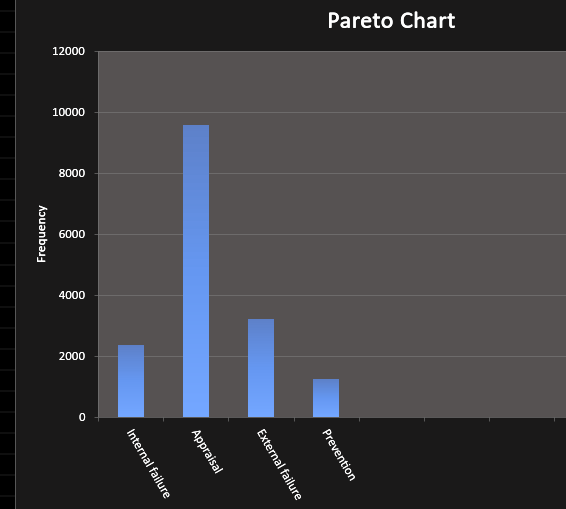
\includegraphics[width=0.5\textwidth]{ /home/matt/niu/fall24/cs466/notes/figures/31.png }
\end{figure}
\noindent
We can see that Appraisal activies appear to be keeping failure costs relatively low; and with better prevention, we can lower them. 


\end{document}
